\documentclass{article}
\usepackage[UTF8]{ctex}
\usepackage{amsmath,amssymb,amstext,amsfonts,mathtools}	%数学排版
\usepackage{graphicx,subfig}							%图形排版
\usepackage{array,multirow,makecell,diagbox}			%表格排版
\usepackage[table]{xcolor}
\usepackage{multicol,float}								%双栏排版
\usepackage{indentfirst}								%段落缩进
\usepackage{textcomp,bm,mathrsfs}						%字体
\usepackage[colorlinks=true,linkcolor=blue,filecolor=magenta,urlcolor=cyan]{hyperref}							%交叉引用
\usepackage{cleveref}
\usepackage{seqsplit}
\usepackage{titlesec}
\usepackage[tc]{titlepic}
\usepackage{cite}
\usepackage{booktabs}
\usepackage[section]{placeins}
\usepackage[a4paper,scale=0.8]{geometry}
\usepackage{fancyhdr}
\usepackage{microtype}
\usepackage{listings}
\usepackage{metalogo}


\setcounter{section}{-1}
\numberwithin{equation}{section}						%公式按章节编号
\numberwithin{figure}{section}							%图表按章节编号

\definecolor{dkgreen}{rgb}{0,0.6,0}
\definecolor{gray}{rgb}{0.5,0.5,0.5}
\definecolor{mauve}{rgb}{0.58,0,0.82}
\lstset{frame=tb,
	language=python,
	xleftmargin=2em,xrightmargin=2em,aboveskip=1em,belowskip=1em,
	showstringspaces=true,
	columns=fullflexible,
	linewidth=1\linewidth, %设置代码块与行同宽
	breaklines=true,%在单词边界处换行
	basicstyle={\small\ttfamily},
	numbers=left,
	%numberstyle=\tiny\courier, %设置行号大小
	numberstyle=\tiny\color{gray},
	keywordstyle=\color{blue},
	commentstyle=\color{dkgreen},
	stringstyle=\color{mauve},
	breaklines=true,
	breakatwhitespace=true,
	escapeinside=``,%逃逸字符(1左面的键),用于显示中文例如在代码中`中文...`
	tabsize=4,
	extendedchars=false %解决代码跨页时,章节标题,页眉等汉字不显示的问题
}
\pagestyle{fancy}

\fancyhead[L]{中国科学技术大学}
\fancyhead[C]{选调生备考}
\fancyhead[R]{2024秋}
\fancyfoot[C]{\thepage}

\newcommand{\upcite}[1]{\textsuperscript{\cite{#1}}}
\renewcommand{\dblfloatpagefraction}{.9}

\titleformat*{\section}{\center\bfseries\Large}
\titleformat*{\subsection}{\bfseries\large}

\newtheorem{definition}{Definition}
\newtheorem{key-point}{Key-point}


\begin{document}
\begin{sloppypar}
	\thispagestyle{empty}
	\begin{center}
		\parbox[t][3cm][c]{\textwidth}{
		\begin{center}
				{\kaishu\Huge 中国科学技术大学}
		\end{center} }
		\parbox[t][8cm][c]{\textwidth}{\huge
		\begin{center} 
				\begin{figure}[H]
					\centering
					
\includegraphics[width=0.4\linewidth]{ustcblue}
				\end{figure}
		\end{center} }
		\parbox[t][2cm][t]{\textwidth}{
		\begin{center}  
				{\kaishu\huge 综合能力测试}
		\end{center} }
		
		\parbox[t][5cm][b]{0.7\textwidth}{
			{\Large\kaishu{PB21020706 姜一夫
\\
					jiangxianchen@mail.ustc.edu.cn
					
} }  }
		
		\parbox[t][5cm][c]{\textwidth}{ {\large
		% \begin{center}
		% 			{\Large\heiti 独立完成声明}
		% 			\\
		% 			本设计根据课程要求阅读材料并认真思考,独立撰写,严格杜绝学术不端行为。(注释掉算了
		% \end{center} 
            } }
	\end{center}
	\clearpage
	

	\newpage\tableofcontents\newpage

\section{Abstract}

一些准备考公的例题和要点总结.(选自980网课)

\textbf{浙江选调考察范围}

\begin{figure}[H]
     \centering
     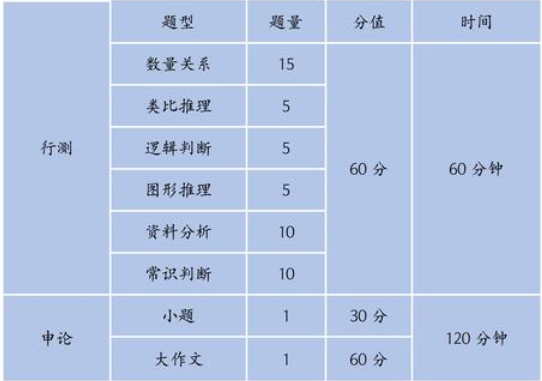
\includegraphics[width=0.6\linewidth]{0.png}
		\caption{浙江选调考察范围}
 \end{figure}

\textbf{安徽选调考察范围}

\begin{figure}[H]
     \centering
     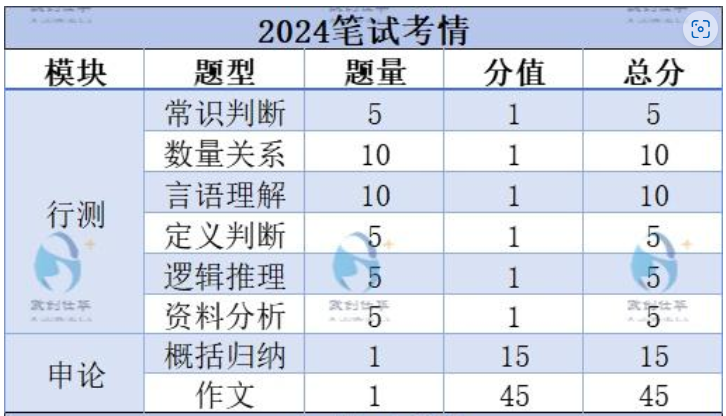
\includegraphics[width=0.6\linewidth]{00.png}
		\caption{安徽选调考察范围}
 \end{figure}

\section{常识判断}






\section{判断推理---图形推理}

\begin{itemize}
    \item 图形推理
    \begin{itemize}
        \item 规律类
\begin{itemize}
    \item 位置类
    \item 样式类
    \item 数量类
    \item 属性类
    \item 功能类
\end{itemize}
        \item 重构类
    
\begin{itemize}
    \item 平面类
    \item 空间类
\end{itemize}
\end{itemize}
\end{itemize}

\subsection{位置类}

\textbf{做题思路:}观察图形特点$\rightarrow$ 锁定相同点和不同点$\rightarrow$猜测可能性考法$\rightarrow$验证并继续猜测


\begin{figure}[H]
     \centering
     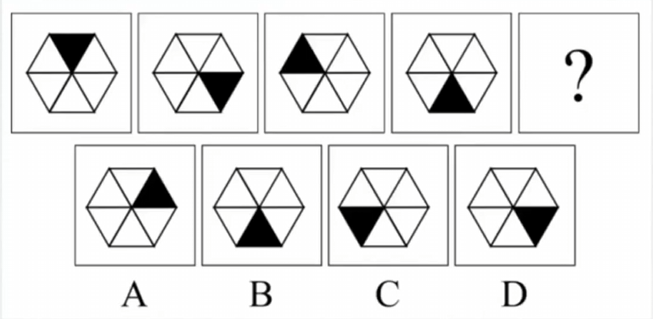
\includegraphics[width=0.5\linewidth]{1.png}
		\caption{Answer:A}
 \end{figure}

\begin{figure}[H]
     \centering
     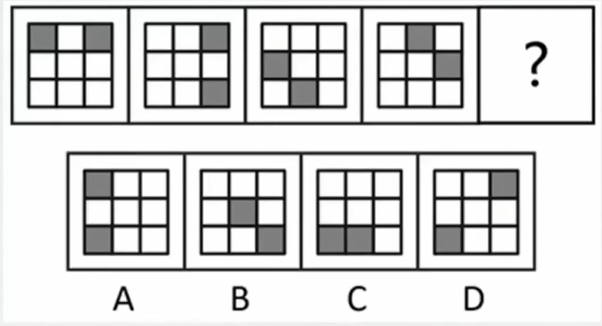
\includegraphics[width=0.5\linewidth]{2.png}
		\caption{Answer:A}
 \end{figure}

\begin{figure}[H]
     \centering
     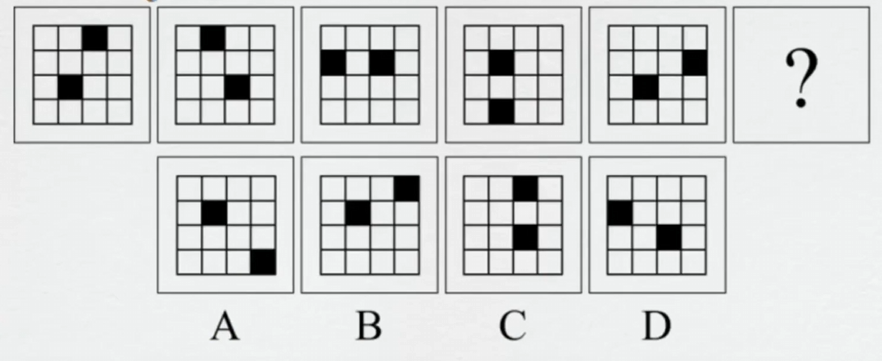
\includegraphics[width=0.5\linewidth]{3.png}
		\caption{Answer:D}
 \end{figure}

\textbf{图1.3:十六宫格注意内外圈}

\begin{figure}[H]
     \centering
     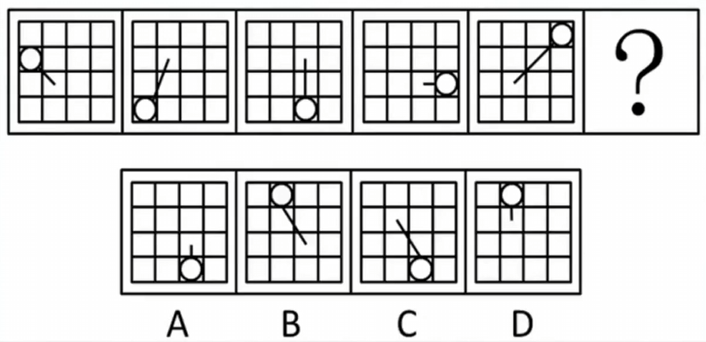
\includegraphics[width=0.5\linewidth]{4.png}
		\caption{Answer:D}
 \end{figure}

\begin{figure}[H]
     \centering
     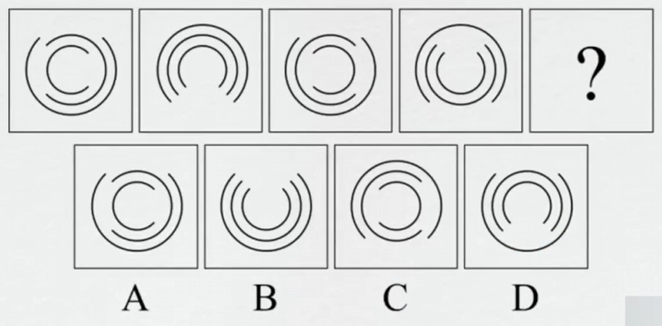
\includegraphics[width=0.5\linewidth]{5.png}
		\caption{Answer:A}
 \end{figure}

\begin{figure}[H]
     \centering
     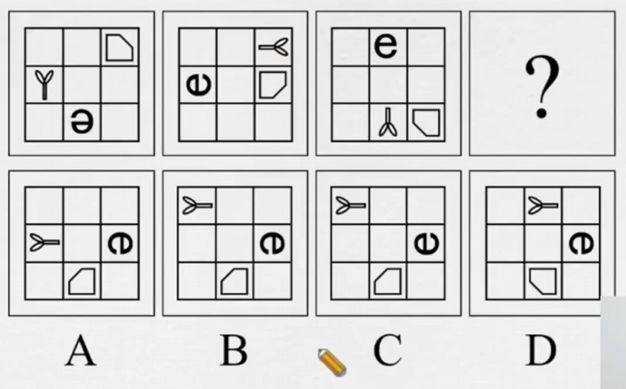
\includegraphics[width=0.5\linewidth]{6.png}
		\caption{Answer:B}
 \end{figure}

\begin{figure}[H]
     \centering
     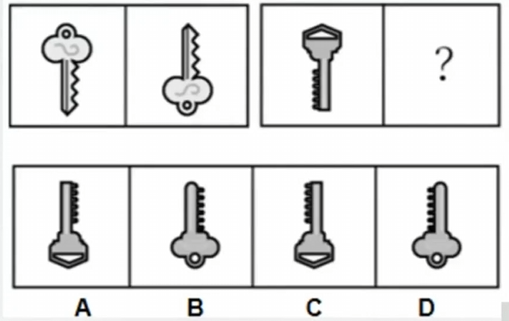
\includegraphics[width=0.5\linewidth]{7.png}
		\caption{Answer:C}
 \end{figure}

\begin{figure}[H]
     \centering
     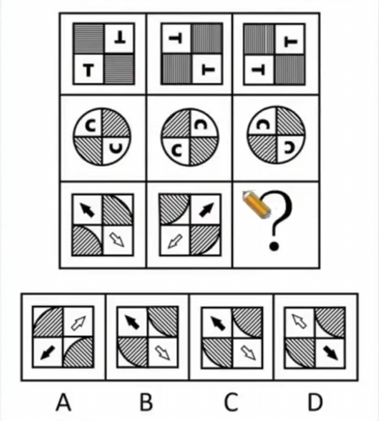
\includegraphics[width=0.5\linewidth]{8.png}
		\caption{Answer:C}
 \end{figure}


\begin{figure}[H]
     \centering
     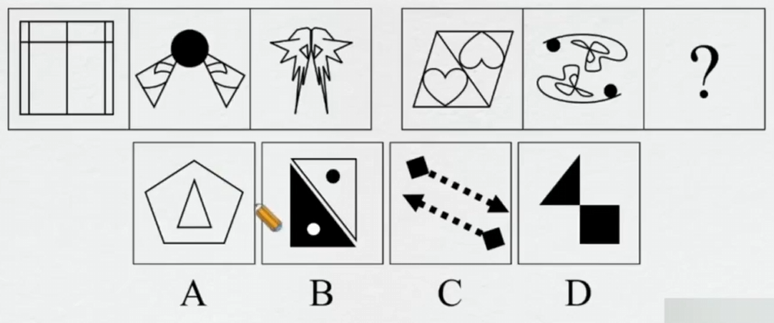
\includegraphics[width=0.5\linewidth]{9.png}
		\caption{Answer:C}
 \end{figure}

\begin{figure}[H]
     \centering
     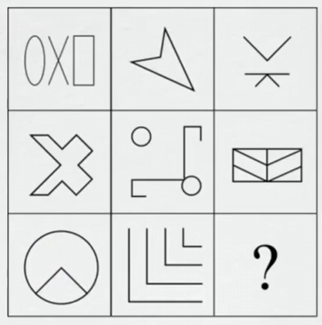
\includegraphics[width=0.5\linewidth]{10.png}
 \end{figure}

\begin{figure}[H]
     \centering
     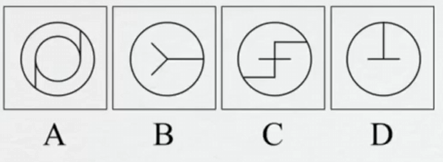
\includegraphics[width=0.5\linewidth]{11.png}
		\caption{Answer:B}
 \end{figure}

\textbf{图1.10:图像存在明显方向指示常考对称性}


\begin{figure}[H]
     \centering
     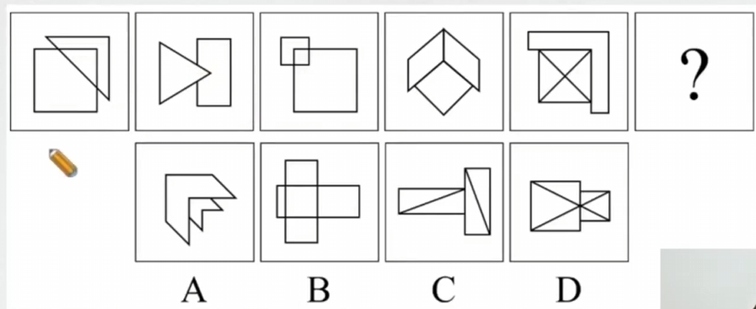
\includegraphics[width=0.5\linewidth]{12.png}
		\caption{Answer:D}
 \end{figure}

\textbf{图1.11:注意对称轴是否经过交点}

\begin{figure}[H]
     \centering
     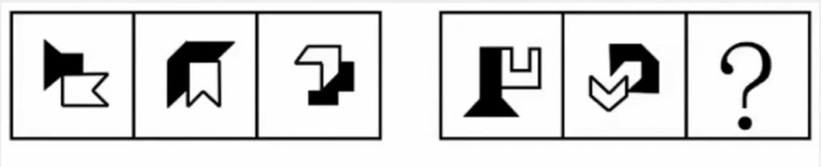
\includegraphics[width=0.5\linewidth]{13.png}
 \end{figure}

\begin{figure}[H]
     \centering
     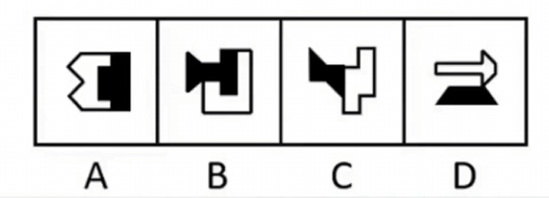
\includegraphics[width=0.3\linewidth]{14.png}
		\caption{Answer:D}
 \end{figure}

\textbf{图1.12:注意对称轴之间夹角}

\begin{figure}[H]
     \centering
     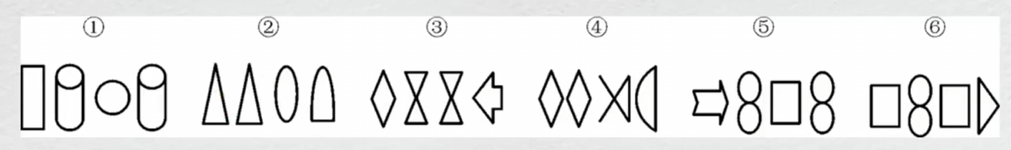
\includegraphics[width=0.65\linewidth]{15.png}
 \end{figure}

\begin{figure}[H]
     \centering
     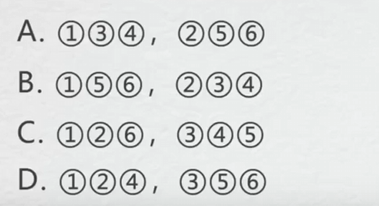
\includegraphics[width=0.25\linewidth]{16.png}
		\caption{Answer:B}
 \end{figure}

\textbf{图1.13:注意相同图形之间的距离(是否挨着)}

\begin{figure}[H]
     \centering
     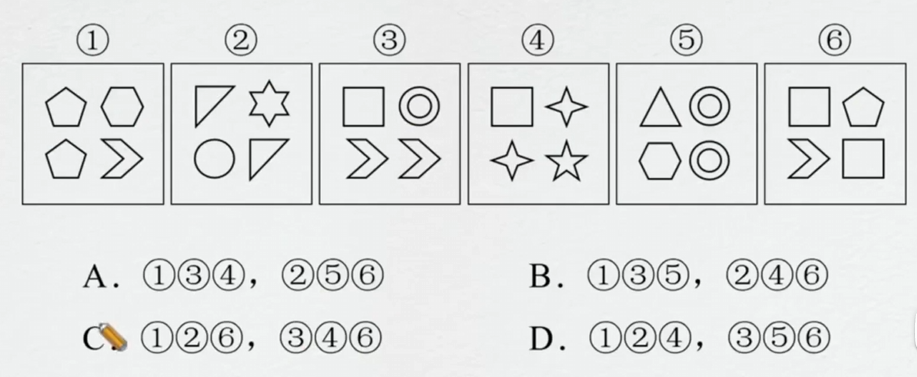
\includegraphics[width=0.5\linewidth]{17.png}
		\caption{Answer:B}
\end{figure}

\begin{figure}[H]
     \centering
     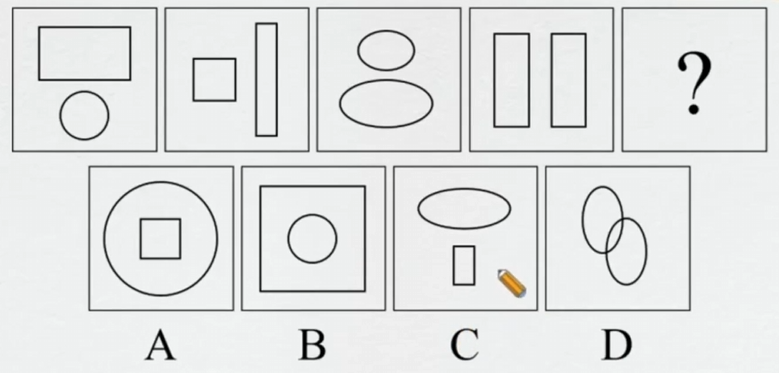
\includegraphics[width=0.5\linewidth]{18.png}
		\caption{Answer:C}
\end{figure}


\begin{figure}[H]
     \centering
     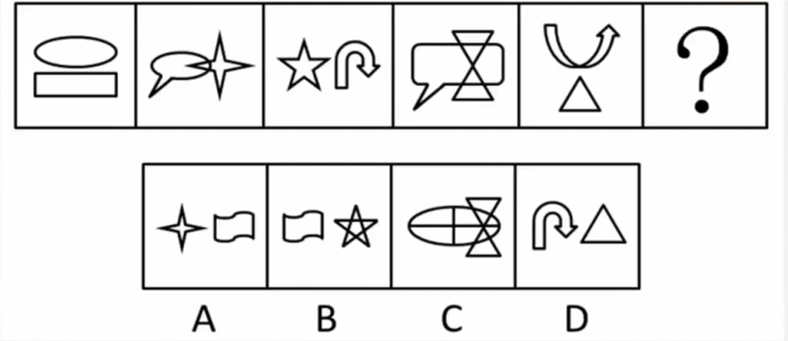
\includegraphics[width=0.5\linewidth]{19.png}
		\caption{Answer:C}
\end{figure}

\begin{figure}[H]
     \centering
     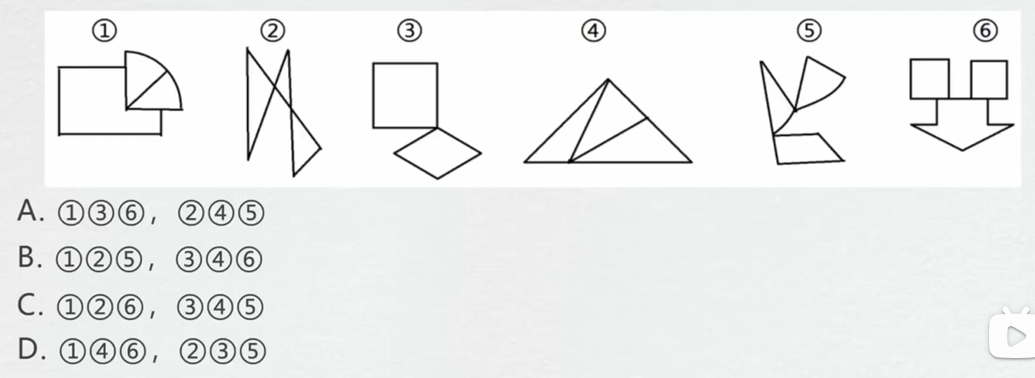
\includegraphics[width=0.55\linewidth]{20.png}
		\caption{Answer:D}
\end{figure}

\textbf{图1.17:注意图形相连接的元素(是点还是线)}

\begin{figure}[H]
     \centering
     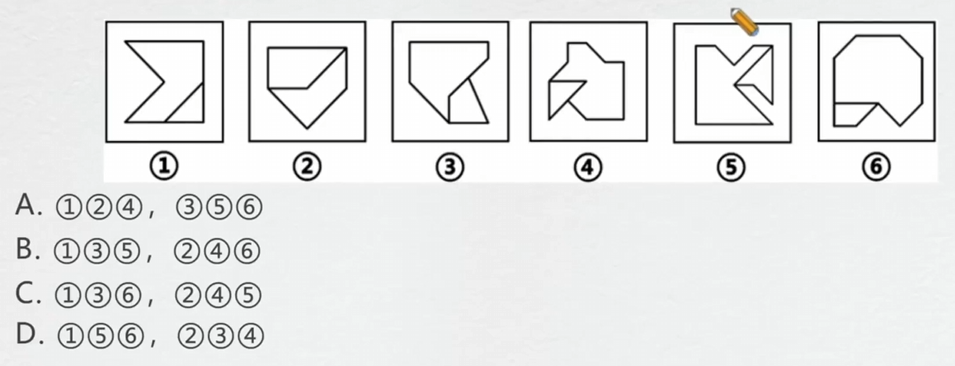
\includegraphics[width=0.55\linewidth]{21.png}
		\caption{Answer:D}
\end{figure}


\begin{figure}[H]
     \centering
     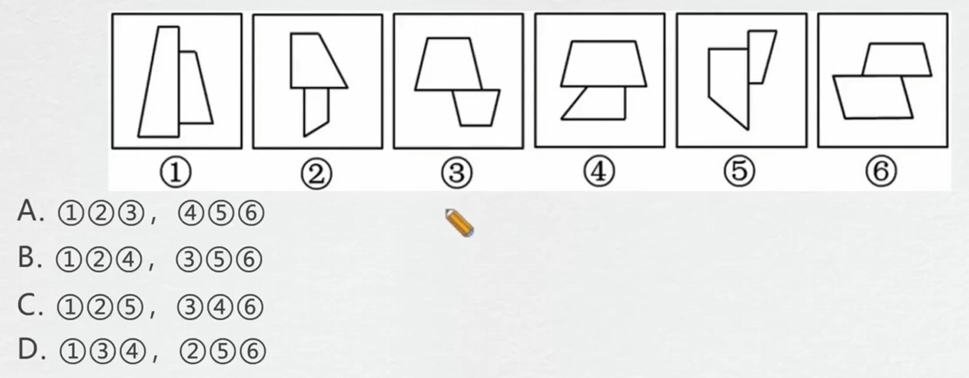
\includegraphics[width=0.55\linewidth]{22.png}
		\caption{Answer:B}
\end{figure}


\begin{figure}[H]
     \centering
     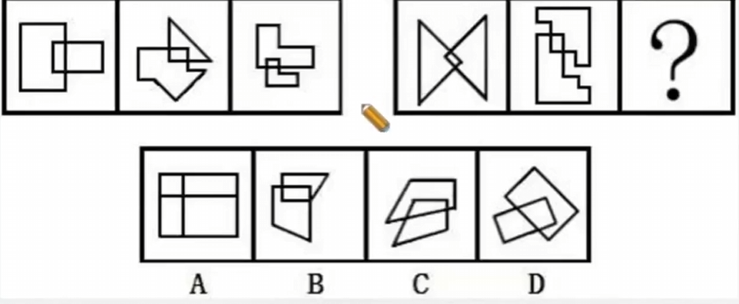
\includegraphics[width=0.55\linewidth]{23.png}
		\caption{Answer:B}
\end{figure}

\begin{figure}[H]
     \centering
     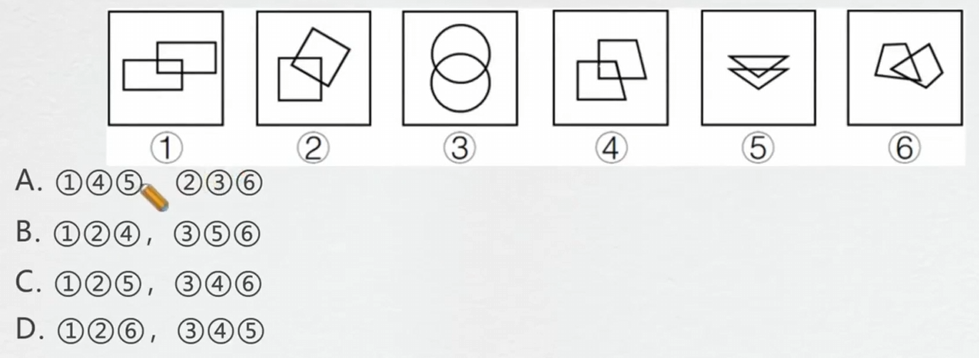
\includegraphics[width=0.6\linewidth]{24.png}
		\caption{Answer:A}
\end{figure}

\textbf{图1.21:特别注意重合的部分}

\begin{figure}[H]
     \centering
     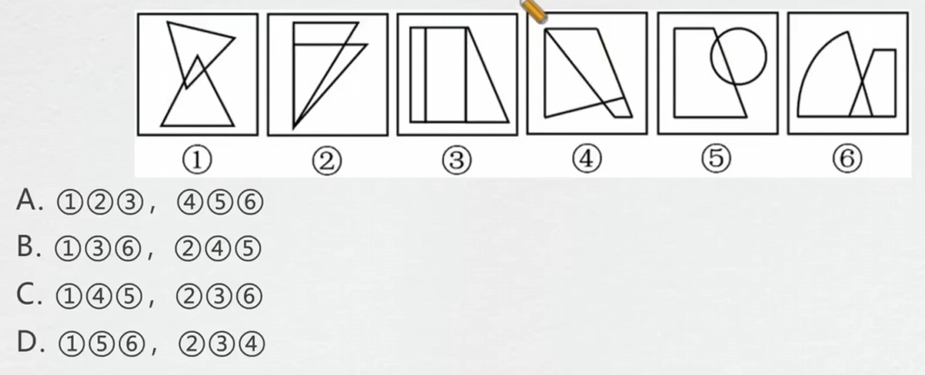
\includegraphics[width=0.6\linewidth]{25.png}
		\caption{Answer:D}
\end{figure}

\textbf{图1.22:特别注意重合部分的面积大小}

\newpage

\subsection{样式类}

\begin{figure}[H]
     \centering
     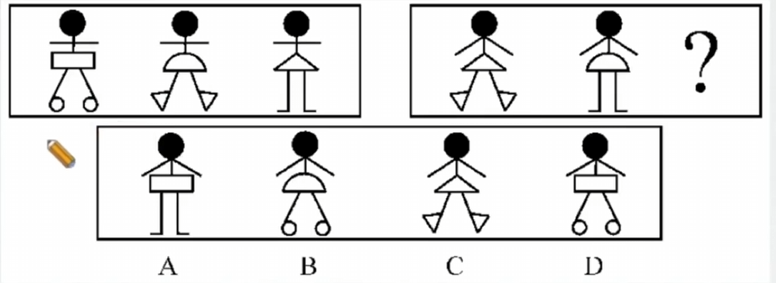
\includegraphics[width=0.6\linewidth]{26.png}
		\caption{Answer:D}
\end{figure}


\begin{figure}[H]
     \centering
     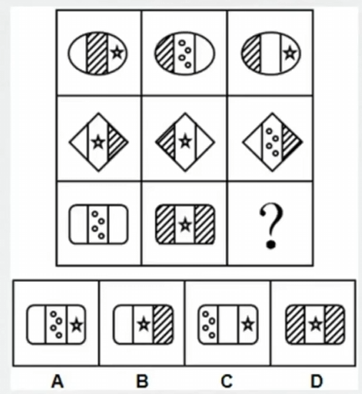
\includegraphics[width=0.35\linewidth]{27.png}
		\caption{Answer:B}
\end{figure}


\begin{figure}[H]
     \centering
     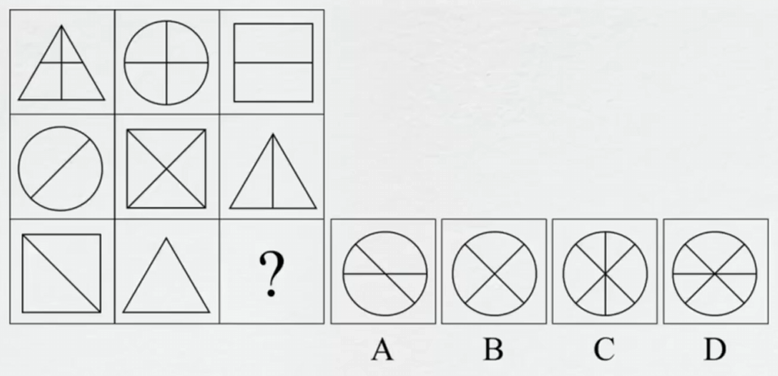
\includegraphics[width=0.5\linewidth]{28.png}
		\caption{Answer:B}
\end{figure}

\textbf{图1.25:注意九宫格竖直方向也可能是规律方向}

\begin{figure}[H]
     \centering
     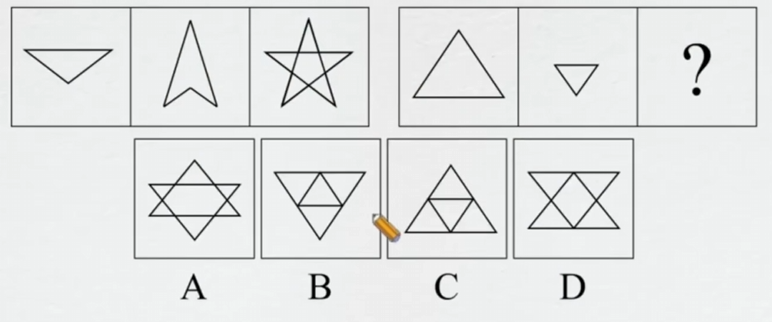
\includegraphics[width=0.5\linewidth]{29.png}
		\caption{Answer:C}
\end{figure}


\begin{figure}[H]
     \centering
     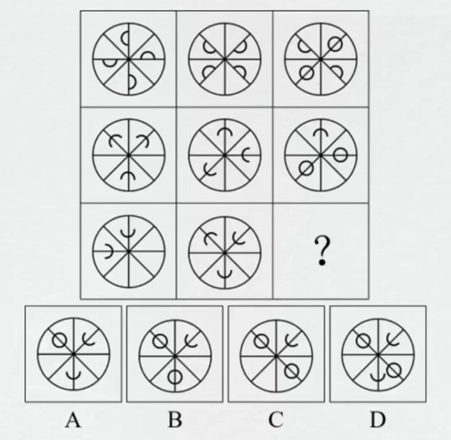
\includegraphics[width=0.5\linewidth]{30.png}
		\caption{Answer:A}
\end{figure}


\begin{figure}[H]
     \centering
     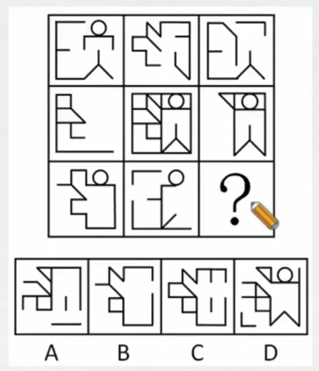
\includegraphics[width=0.35\linewidth]{31.png}
		\caption{Answer:B}
\end{figure}

\textbf{图1.28:注意当九宫格中心图形复杂时考虑米字型结构}

\begin{figure}[H]
     \centering
     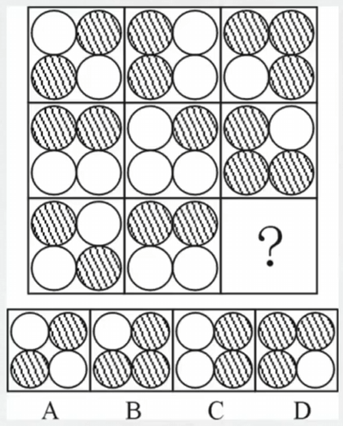
\includegraphics[width=0.35\linewidth]{32.png}
		\caption{Answer:B}
\end{figure}

\begin{figure}[H]
     \centering
     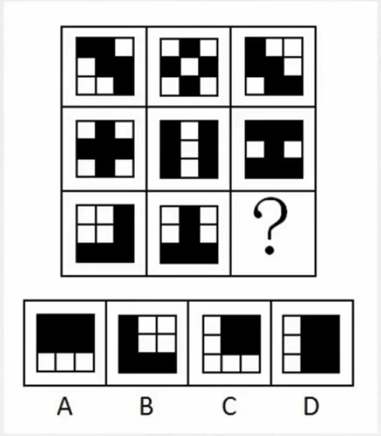
\includegraphics[width=0.35\linewidth]{33.png}
		\caption{Answer:C}
\end{figure}

\begin{figure}[H]
     \centering
     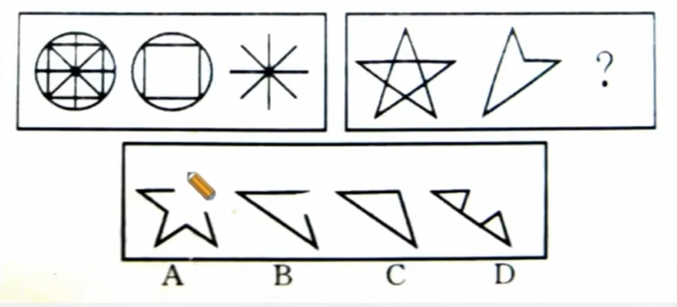
\includegraphics[width=0.5\linewidth]{34.png}
		\caption{Answer:C}
\end{figure}

\begin{figure}[H]
     \centering
     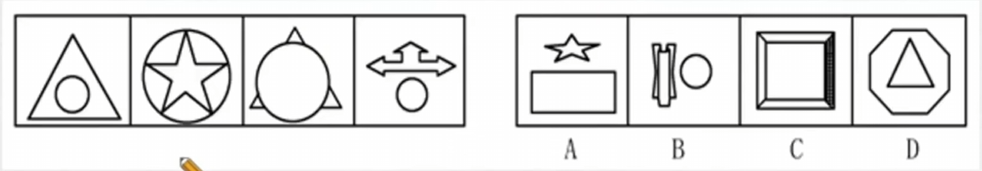
\includegraphics[width=0.65\linewidth]{35.png}
		\caption{Answer:B}
\end{figure}

\textbf{图1.32:注意考虑所有图的共同点或是相邻图的共同点}

\begin{figure}[H]
     \centering
     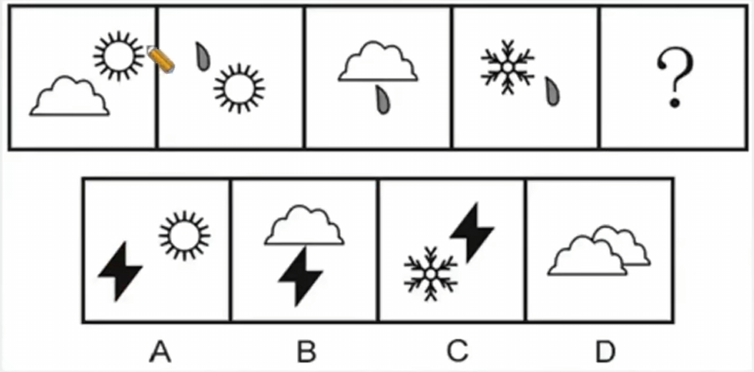
\includegraphics[width=0.5\linewidth]{36.png}
		\caption{Answer:C}
\end{figure}


\begin{figure}[H]
     \centering
     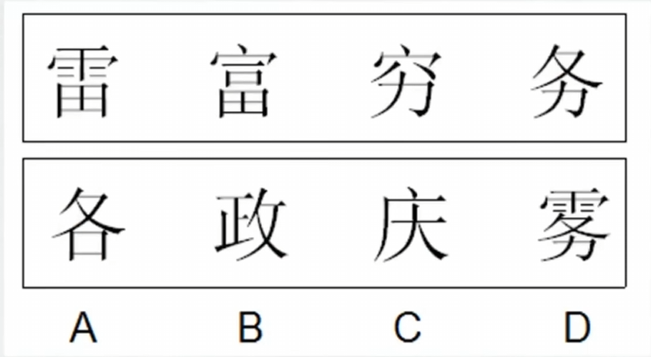
\includegraphics[width=0.5\linewidth]{37.png}
		\caption{Answer:A}
\end{figure}


\begin{figure}[H]
     \centering
     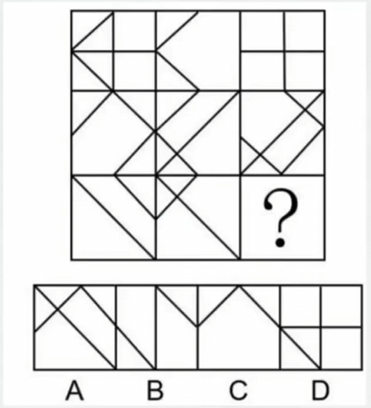
\includegraphics[width=0.4\linewidth]{38.png}
		\caption{Answer:C}
\end{figure}


\begin{figure}[H]
     \centering
     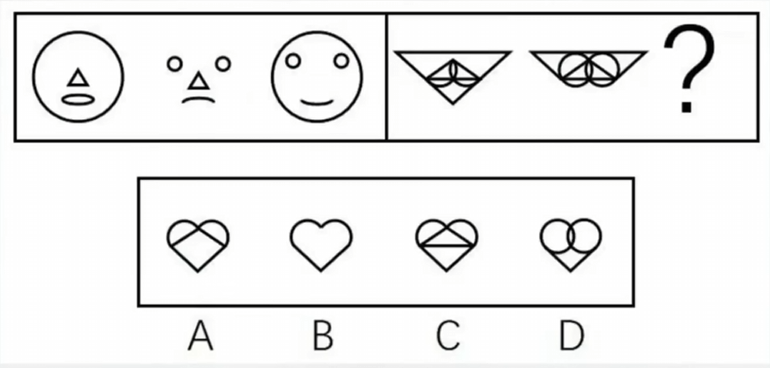
\includegraphics[width=0.5\linewidth]{39.png}
		\caption{Answer:B}
\end{figure}


\begin{figure}[H]
     \centering
     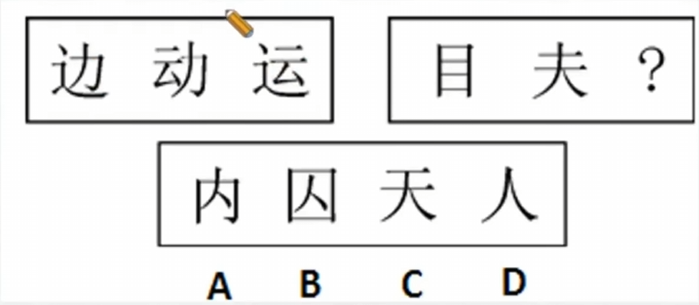
\includegraphics[width=0.5\linewidth]{40.png}
		\caption{Answer:B}
\end{figure}

\begin{figure}[H]
     \centering
     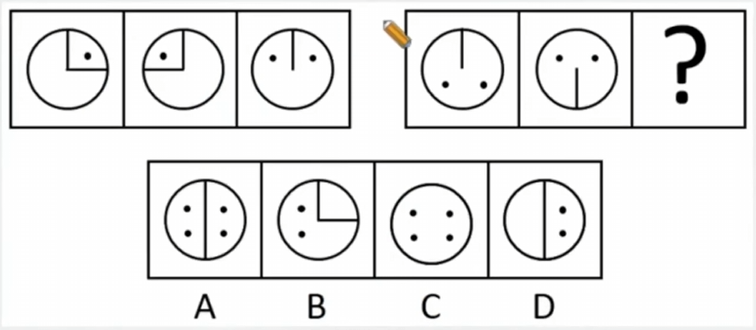
\includegraphics[width=0.5\linewidth]{41.png}
		\caption{Answer:C}
\end{figure}


\begin{figure}[H]
     \centering
     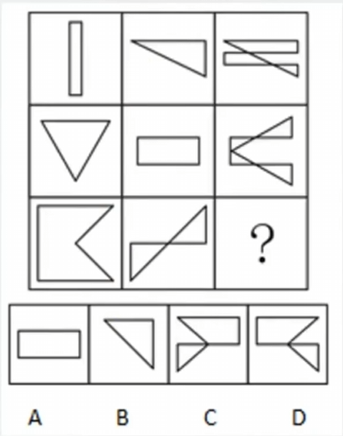
\includegraphics[width=0.35\linewidth]{42.png}
		\caption{Answer:D}
\end{figure}

\subsection{数量类}

\textbf{此类题目往往组成元素混乱}


\begin{figure}[H]
     \centering
     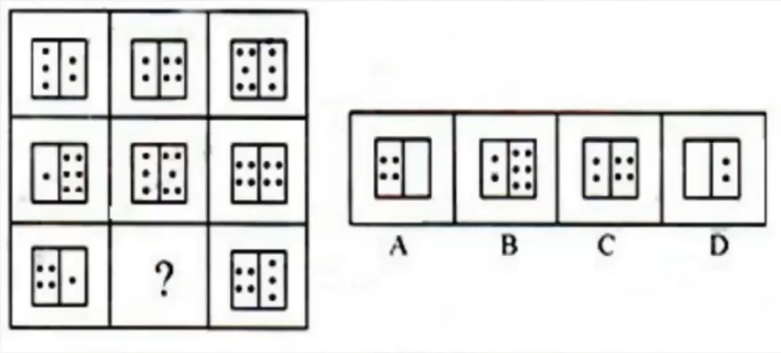
\includegraphics[width=0.5\linewidth]{43.png}
		\caption{Answer:D}
\end{figure}

\textbf{图1.40:注意九宫格类图形目标列不一定是第三列,也可能是中间列}

\begin{figure}[H]
     \centering
     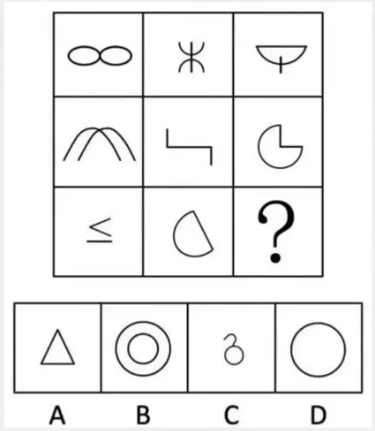
\includegraphics[width=0.35\linewidth]{44.png}
		\caption{Answer:A}
\end{figure}


\begin{figure}[H]
     \centering
     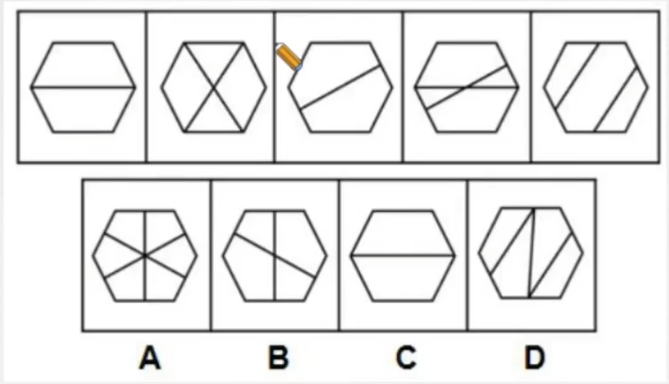
\includegraphics[width=0.45\linewidth]{45.png}
		\caption{Answer:B}
\end{figure}

\textbf{图1.42:注意外侧原顶点和交点之和}


\begin{figure}[H]
     \centering
     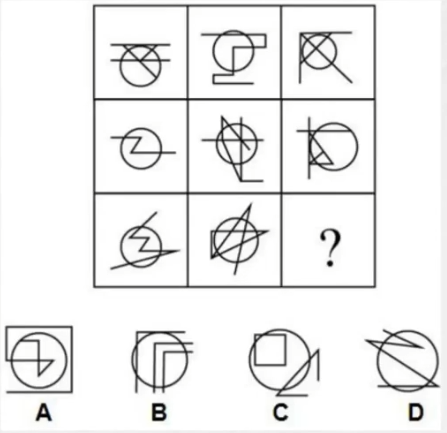
\includegraphics[width=0.45\linewidth]{46.png}
		\caption{Answer:C}
\end{figure}



\begin{figure}[H]
     \centering
     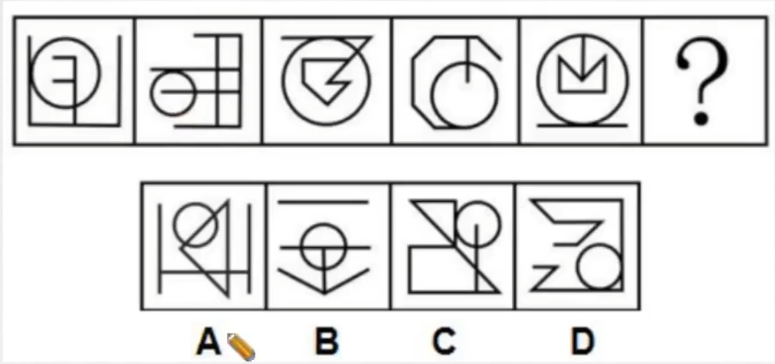
\includegraphics[width=0.5\linewidth]{47.png}
		\caption{Answer:C}
\end{figure}


\begin{figure}[H]
     \centering
     \includegraphics[width=0.5\linewidth]{48.png}
		\caption{Answer:C}
\end{figure}


\begin{figure}[H]
     \centering
     \includegraphics[width=0.55\linewidth]{49.png}
		\caption{Answer:A}
\end{figure}


\begin{figure}[H]
     \centering
     \includegraphics[width=0.6\linewidth]{50.png}
		\caption{Answer:C}
\end{figure}


\begin{figure}[H]
     \centering
     \includegraphics[width=0.6\linewidth]{51.png}
		\caption{Answer:D}
\end{figure}


\begin{figure}[H]
     \centering
     \includegraphics[width=0.6\linewidth]{52.png}
		\caption{Answer:C}
\end{figure}



\begin{figure}[H]
     \centering
     \includegraphics[width=0.6\linewidth]{53.png}
		\caption{Answer:A}
\end{figure}


\begin{figure}[H]
     \centering
     \includegraphics[width=0.6\linewidth]{54.png}
		\caption{Answer:B}
\end{figure}


\begin{figure}[H]
     \centering
     \includegraphics[width=0.6\linewidth]{55.png}
		\caption{Answer:D}
\end{figure}

\textbf{图1.52:注意某些定义下的线数量}


\begin{figure}[H]
     \centering
     \includegraphics[width=0.6\linewidth]{56.png}
		\caption{Answer:D}
\end{figure}

\begin{figure}[H]
     \centering
     \includegraphics[width=0.6\linewidth]{57.png}
		\caption{Answer:D}
\end{figure}

\textbf{图1.54:注意折线的首尾方向(相反)}


\begin{figure}[H]
     \centering
     \includegraphics[width=0.75\linewidth]{58.png}
		\caption{Answer:B}
\end{figure}


\begin{figure}[H]
     \centering
     \includegraphics[width=0.6\linewidth]{59.png}
		\caption{Answer:D}
\end{figure}

\textbf{图1.56:注意图中曲线数量}


\begin{figure}[H]
     \centering
     \includegraphics[width=0.6\linewidth]{60.png}
		\caption{Answer:A}
\end{figure}


\textbf{图1.57:注意图形覆盖产生的主客体关系}


\begin{figure}[H]
     \centering
     \includegraphics[width=0.6\linewidth]{61.png}
		\caption{Answer:A}
\end{figure}

\textbf{图1.58:注意曲线和直线的数量之差}

\begin{figure}[H]
     \centering
     \includegraphics[width=0.6\linewidth]{62.png}
		\caption{Answer:B}
\end{figure}

\textbf{图1.59:注意直线数量产生的数量关系(是否需要计算加工)}

\begin{figure}[H]
     \centering
     \includegraphics[width=0.6\linewidth]{63.png}
		\caption{Answer:D}
\end{figure}

\textbf{图1.60:注意奇点定义与计算方法}

\begin{figure}[H]
     \centering
     \includegraphics[width=0.6\linewidth]{64.png}
		\caption{Answer:C}
\end{figure}


\begin{figure}[H]
     \centering
     \includegraphics[width=0.45\linewidth]{65.png}
		\caption{Answer:D}
\end{figure}


\begin{figure}[H]
     \centering
     \includegraphics[width=0.6\linewidth]{66.png}
		\caption{Answer:C}
\end{figure}


\begin{figure}[H]
     \centering
     \includegraphics[width=0.45\linewidth]{67.png}
		\caption{Answer:B}
\end{figure}


\begin{figure}[H]
     \centering
     \includegraphics[width=0.6\linewidth]{68.png}
		\caption{Answer:D}
\end{figure}


\textbf{图1.65:注意只考虑元素存在性不考虑数量}

\begin{figure}[H]
     \centering
     \includegraphics[width=0.4\linewidth]{69.png}
		\caption{Answer:D}
\end{figure}


\begin{figure}[H]
     \centering
     \includegraphics[width=0.6\linewidth]{70.png}
		\caption{Answer:B}
\end{figure}

\begin{figure}[H]
     \centering
     \includegraphics[width=0.6\linewidth]{71.png}
		\caption{Answer:C}
\end{figure}

\textbf{图1.68:注意对于面的定义,需要封闭性}

\begin{figure}[H]
     \centering
     \includegraphics[width=0.6\linewidth]{72.png}
		\caption{Answer:C}
\end{figure}


\begin{figure}[H]
     \centering
     \includegraphics[width=0.6\linewidth]{73.png}
		\caption{Answer:B}
\end{figure}

\begin{figure}[H]
     \centering
     \includegraphics[width=0.6\linewidth]{74.png}
		\caption{Answer:D}
\end{figure}

\begin{figure}[H]
     \centering
     \includegraphics[width=0.6\linewidth]{75.png}
		\caption{Answer:B}
\end{figure}


\begin{figure}[H]
     \centering
     \includegraphics[width=0.6\linewidth]{76.png}
		\caption{Answer:D}
\end{figure}

\textbf{图1.73:注意切割后的面本身性质}


\begin{figure}[H]
     \centering
     \includegraphics[width=0.6\linewidth]{77.png}
		\caption{Answer:D}
\end{figure}


\begin{figure}[H]
     \centering
     \includegraphics[width=0.6\linewidth]{78.png}
		\caption{Answer:C}
\end{figure}

\textbf{图1.75:注意切割后最大面和最小面的形状}

\begin{figure}[H]
     \centering
     \includegraphics[width=0.6\linewidth]{79.png}
		\caption{Answer:C}
\end{figure}

\textbf{图1.76:注意切割后最大面和最小面以及整体图形的形状关系}

\begin{figure}[H]
     \centering
     \includegraphics[width=0.6\linewidth]{80.png}
		\caption{Answer:C}
\end{figure}




\begin{figure}[H]
     \centering
     \includegraphics[width=0.6\linewidth]{81.png}
		\caption{Answer:D}
\end{figure}

\textbf{图1.78:注意素本身的数量(也即黑色部分的数量)}


\begin{figure}[H]
     \centering
     \includegraphics[width=0.6\linewidth]{82.png}
		\caption{Answer:C}
\end{figure}



\begin{figure}[H]
     \centering
     \includegraphics[width=0.6\linewidth]{83.png}
		\caption{Answer:B}
\end{figure}


\begin{figure}[H]
     \centering
     \includegraphics[width=0.6\linewidth]{84.png}
		\caption{Answer:A}
\end{figure}


\begin{figure}[H]
     \centering
     \includegraphics[width=0.6\linewidth]{85.png}
		\caption{Answer:D}
\end{figure}


\begin{figure}[H]
     \centering
     \includegraphics[width=0.6\linewidth]{86.png}
		\caption{Answer:D}
\end{figure}

\textbf{图1.83:注意当多元素数量各自没有明显规律时考虑它们之间运算后得到的结果}

\begin{figure}[H]
     \centering
     \includegraphics[width=0.6\linewidth]{87.png}
		\caption{Answer:A}
\end{figure}


\begin{figure}[H]
     \centering
     \includegraphics[width=0.6\linewidth]{88.png}
		\caption{Answer:B}
\end{figure}


\subsection{六面体}


\begin{figure}[H]
     \centering
     \includegraphics[width=0.6\linewidth]{89.png}
		\caption{Answer:B}
\end{figure}

\begin{figure}[H]
     \centering
     \includegraphics[width=0.4\linewidth]{91.png}
\end{figure}

\begin{figure}[H]
     \centering
     \includegraphics[width=0.3\linewidth]{90.png}
		\caption{Answer:D}
\end{figure}



\begin{figure}[H]
     \centering
     \includegraphics[width=0.6\linewidth]{92.png}
		
\end{figure}

\begin{figure}[H]
     \centering
     \includegraphics[width=0.6\linewidth]{93.png}
		\caption{Answer:C}
\end{figure}


\begin{figure}[H]
     \centering
     \includegraphics[width=0.6\linewidth]{94.png}
	
\end{figure}

\begin{figure}[H]
     \centering
     \includegraphics[width=0.6\linewidth]{95.png}
		\caption{Answer:B}
\end{figure}


\begin{figure}[H]
     \centering
     \includegraphics[width=0.6\linewidth]{96.png}
		\caption{Answer:C}
\end{figure}


\begin{figure}[H]
     \centering
     \includegraphics[width=0.6\linewidth]{97.png}
		\caption{Answer:B}
\end{figure}


\begin{figure}[H]
     \centering
     \includegraphics[width=0.6\linewidth]{98.png}
		\caption{Answer:A}
\end{figure}

\begin{figure}[H]
     \centering
     \includegraphics[width=0.6\linewidth]{99.png}
		\caption{Answer:D}
\end{figure}


\section{判断推理---类比推理}


\textbf{题目示例:}

\begin{figure}[H]
     \centering
     \includegraphics[width=0.6\linewidth]{100.png}
\end{figure}


\textbf{解题方法:词性/逻辑关系/其他关系}


\begin{itemize}

	\item 
外延关系

\item
内涵关系

\item
语法关系

\item
语义关系

\end{itemize}


\subsection{外延关系}


\begin{figure}[H]
     \centering
     \includegraphics[width=0.4\linewidth]{101.png}
		\caption{Answer:D}
\end{figure}


\begin{figure}[H]
     \centering
     \includegraphics[width=0.4\linewidth]{102.png}
		\caption{Answer:D}
\end{figure}

\textbf{羊城:广州/江城:武汉/申城:上海/煤城:大同/龙城:太原/泉城:济南}

\begin{figure}[H]
     \centering
     \includegraphics[width=0.4\linewidth]{103.png}
		\caption{Answer:B}
\end{figure}


\begin{figure}[H]
     \centering
     \includegraphics[width=0.4\linewidth]{104.png}
		\caption{Answer:C}
\end{figure}

\textbf{图2.4:注意并列关系时选项的总和是否为全集}

\begin{figure}[H]
     \centering
     \includegraphics[width=0.4\linewidth]{105.png}
		\caption{Answer:C}
\end{figure}


\begin{figure}[H]
     \centering
     \includegraphics[width=0.4\linewidth]{106.png}
		\caption{Answer:A}
\end{figure}


\begin{figure}[H]
     \centering
     \includegraphics[width=0.4\linewidth]{107.png}
		\caption{Answer:C}
\end{figure}


\begin{figure}[H]
     \centering
     \includegraphics[width=0.4\linewidth]{108.png}
		\caption{Answer:C}
\end{figure}


\begin{figure}[H]
     \centering
     \includegraphics[width=0.4\linewidth]{109.png}
		\caption{Answer:B}
\end{figure}


\begin{figure}[H]
     \centering
     \includegraphics[width=0.4\linewidth]{110.png}
		\caption{Answer:C}
\end{figure}


\begin{figure}[H]
     \centering
     \includegraphics[width=0.4\linewidth]{111.png}
		\caption{Answer:B}
\end{figure}


\begin{figure}[H]
     \centering
     \includegraphics[width=0.4\linewidth]{112.png}
		\caption{Answer:C}
\end{figure}


\begin{figure}[H]
     \centering
     \includegraphics[width=0.4\linewidth]{113.png}
		\caption{Answer:C}
\end{figure}


\begin{figure}[H]
     \centering
     \includegraphics[width=0.4\linewidth]{114.png}
		\caption{Answer:C}
\end{figure}


\begin{figure}[H]
     \centering
     \includegraphics[width=0.4\linewidth]{115.png}
		\caption{Answer:A}
\end{figure}


\begin{figure}[H]
     \centering
     \includegraphics[width=0.4\linewidth]{116.png}
		\caption{Answer:C}
\end{figure}

\textbf{腔肠动物和软体动物是并列关系/甲壳纲动物和节肢动物是属于关系}

\begin{figure}[H]
     \centering
     \includegraphics[width=0.4\linewidth]{117.png}
		\caption{Answer:C}
\end{figure}


\subsection{内涵关系}



\begin{figure}[H]
     \centering
     \includegraphics[width=0.4\linewidth]{118.png}
		\caption{Answer:A}
\end{figure}


\begin{figure}[H]
     \centering
     \includegraphics[width=0.4\linewidth]{119.png}
		\caption{Answer:C}
\end{figure}


\begin{figure}[H]
     \centering
     \includegraphics[width=0.4\linewidth]{120.png}
		\caption{Answer:B}
\end{figure}


\begin{figure}[H]
     \centering
     \includegraphics[width=0.4\linewidth]{121.png}
		\caption{Answer:B}
\end{figure}


\begin{figure}[H]
     \centering
     \includegraphics[width=0.4\linewidth]{122.png}
		\caption{Answer:C}
\end{figure}


\begin{figure}[H]
     \centering
     \includegraphics[width=0.4\linewidth]{123.png}
		\caption{Answer:C}
\end{figure}

\textbf{图2.23:考虑是否是充分条件/考虑时间顺序(事件发生顺序)}

\begin{figure}[H]
     \centering
     \includegraphics[width=0.4\linewidth]{124.png}
		\caption{Answer:B}
\end{figure}


\begin{figure}[H]
     \centering
     \includegraphics[width=0.4\linewidth]{125.png}
		\caption{Answer:D}
\end{figure}


\begin{figure}[H]
     \centering
     \includegraphics[width=0.4\linewidth]{126.png}
		\caption{Answer:A}
\end{figure}

\begin{figure}[H]
     \centering
     \includegraphics[width=0.4\linewidth]{127.png}
		\caption{Answer:A}
\end{figure}

\begin{figure}[H]
     \centering
     \includegraphics[width=0.4\linewidth]{128.png}
		\caption{Answer:D}
\end{figure}


\begin{figure}[H]
     \centering
     \includegraphics[width=0.4\linewidth]{129.png}
		\caption{Answer:B}
\end{figure}

\subsection{语义关系}

\begin{figure}[H]
     \centering
     \includegraphics[width=0.4\linewidth]{130.png}
		\caption{Answer:C}
\end{figure}

\begin{figure}[H]
     \centering
     \includegraphics[width=0.4\linewidth]{131.png}
		\caption{Answer:A}
\end{figure}

\begin{figure}[H]
     \centering
     \includegraphics[width=0.4\linewidth]{132.png}
		\caption{Answer:D}
\end{figure}


\begin{figure}[H]
     \centering
     \includegraphics[width=0.4\linewidth]{133.png}
		\caption{Answer:C}
\end{figure}

\begin{figure}[H]
     \centering
     \includegraphics[width=0.4\linewidth]{134.png}
		\caption{Answer:A}
\end{figure}


\begin{figure}[H]
     \centering
     \includegraphics[width=0.4\linewidth]{135.png}
		\caption{Answer:B}
\end{figure}

\textbf{图2.35:考虑成语自身的结构中字的词性和关系}

\begin{figure}[H]
     \centering
     \includegraphics[width=0.4\linewidth]{136.png}
		\caption{Answer:A}
\end{figure}


\begin{figure}[H]
     \centering
     \includegraphics[width=0.4\linewidth]{137.png}
		\caption{Answer:B}
\end{figure}


\begin{figure}[H]
     \centering
     \includegraphics[width=0.4\linewidth]{138.png}
		\caption{Answer:D}
\end{figure}

\begin{figure}[H]
     \centering
     \includegraphics[width=0.4\linewidth]{139.png}
		\caption{Answer:D}
\end{figure}


\begin{figure}[H]
     \centering
     \includegraphics[width=0.4\linewidth]{140.png}
		\caption{Answer:D}
\end{figure}

\subsection{语法关系}

\begin{figure}[H]
     \centering
     \includegraphics[width=0.4\linewidth]{141.png}
		\caption{Answer:B}
\end{figure}


\begin{figure}[H]
     \centering
     \includegraphics[width=0.4\linewidth]{142.png}
		\caption{Answer:B}
\end{figure}

\begin{figure}[H]
     \centering
     \includegraphics[width=0.4\linewidth]{143.png}
		\caption{Answer:D}
\end{figure}

\begin{figure}[H]
     \centering
     \includegraphics[width=0.4\linewidth]{144.png}
		\caption{Answer:B}
\end{figure}


\begin{figure}[H]
     \centering
     \includegraphics[width=0.4\linewidth]{145.png}
		\caption{Answer:B}
\end{figure}

\begin{figure}[H]
     \centering
     \includegraphics[width=0.4\linewidth]{146.png}
		\caption{Answer:D}
\end{figure}


\subsection{定义判断}



\section{判断推理---逻辑判断}



\subsection{翻译推理}

\textbf{和逻辑命题相关度很高}

\begin{figure}[H]
     \centering
     \includegraphics[width=0.4\linewidth]{147.png}
\end{figure}

\subsubsection{假言命题}


\begin{figure}[H]
     \centering
     \includegraphics[width=0.4\linewidth]{148.png}
	\caption{假言命题}
\end{figure}



\begin{figure}[H]
     \centering
     \includegraphics[width=0.4\linewidth]{149.png}
	\caption{假言命题}
\end{figure}


\begin{figure}[H]
     \centering
     \includegraphics[width=0.6\linewidth]{150.png}
	\caption{Answer:C}
\end{figure}



\begin{figure}[H]
     \centering
     \includegraphics[width=0.6\linewidth]{151.png}
	\caption{Answer:C}
\end{figure}


\textbf{常用表达:}

\begin{figure}[H]
     \centering
     \includegraphics[width=0.6\linewidth]{152.png}
\end{figure}


\begin{figure}[H]
     \centering
     \includegraphics[width=0.6\linewidth]{153.png}
\end{figure}


\begin{figure}[H]
     \centering
     \includegraphics[width=0.6\linewidth]{154.png}
	\caption{Answer:C}
\end{figure}

\begin{figure}[H]
     \centering
     \includegraphics[width=0.6\linewidth]{155.png}
\end{figure}

\begin{figure}[H]
     \centering
     \includegraphics[width=0.6\linewidth]{156.png}
	\caption{Answer:A}
\end{figure}


\textbf{图2.52:此题中A/D为逆否命题,但是需要注意因果关系$\neq$逻辑关系,因为存在时间顺序}

\begin{figure}[H]
     \centering
     \includegraphics[width=0.6\linewidth]{157.png}
	\caption{Answer:D}
\end{figure}

\textbf{图2.53:注意此题中的递推关系}


\subsubsection{联言选言}

\begin{figure}[H]
     \centering
     \includegraphics[width=0.35\linewidth]{158.png}
\end{figure}


\begin{figure}[H]
     \centering
     \includegraphics[width=0.35\linewidth]{159.png}
\end{figure}


\begin{figure}[H]
     \centering
     \includegraphics[width=0.35\linewidth]{160.png}
\end{figure}

\begin{figure}[H]
     \centering
     \includegraphics[width=0.6\linewidth]{161.png}
	\caption{Answer:C}
\end{figure}


\begin{figure}[H]
     \centering
     \includegraphics[width=0.45\linewidth]{162.png}
	\caption{Answer:B}
\end{figure}


\textbf{总结}

\begin{figure}[H]
     \centering
     \includegraphics[width=0.65\linewidth]{163.png}
\end{figure}





\subsection{真假推理}

\begin{figure}[H]
     \centering
     \includegraphics[width=0.6\linewidth]{164.png}
\end{figure}


\subsubsection{矛盾}


\begin{figure}[H]
     \centering
     \includegraphics[width=0.6\linewidth]{165.png}
\end{figure}


\begin{figure}[H]
     \centering
     \includegraphics[width=0.6\linewidth]{166.png}
\end{figure}


\begin{figure}[H]
     \centering
     \includegraphics[width=0.45\linewidth]{167.png}
		\caption{Answer:B}
\end{figure}


\begin{figure}[H]
     \centering
     \includegraphics[width=0.6\linewidth]{168.png}
\end{figure}


\begin{figure}[H]
     \centering
     \includegraphics[width=0.35\linewidth]{169.png}
		\caption{Answer:C}
\end{figure}


\textbf{图4.2:注意寻找矛盾条件,真命题必在矛盾条件中,意味着其他条件真假性确定}


\begin{figure}[H]
     \centering
     \includegraphics[width=0.6\linewidth]{170.png}
\end{figure}

\begin{figure}[H]
     \centering
     \includegraphics[width=0.5\linewidth]{171.png}
		\caption{Answer:A}
\end{figure}


\begin{figure}[H]
     \centering
     \includegraphics[width=0.6\linewidth]{172.png}
\end{figure}


\begin{figure}[H]
     \centering
     \includegraphics[width=0.5\linewidth]{173.png}
		\caption{Answer:D}
\end{figure}


\subsubsection{反对}


\begin{figure}[H]
     \centering
     \includegraphics[width=0.4\linewidth]{174.png}
\end{figure}


\begin{figure}[H]
     \centering
     \includegraphics[width=0.3\linewidth]{175.png}
\end{figure}

\begin{figure}[H]
     \centering
     \includegraphics[width=0.6\linewidth]{176.png}
		\caption{Answer:B}
\end{figure}


\begin{figure}[H]
     \centering
     \includegraphics[width=0.6\linewidth]{177.png}
	
\end{figure}

\begin{figure}[H]
     \centering
     \includegraphics[width=0.3\linewidth]{178.png}
		\caption{Answer:D}
\end{figure}

\begin{figure}[H]
     \centering
     \includegraphics[width=0.6\linewidth]{179.png}
	
\end{figure}

\begin{figure}[H]
     \centering
     \includegraphics[width=0.35\linewidth]{180.png}
		\caption{Answer:A}
\end{figure}


\begin{figure}[H]
     \centering
     \includegraphics[width=0.6\linewidth]{181.png}
	
\end{figure}

\begin{figure}[H]
     \centering
     \includegraphics[width=0.4\linewidth]{182.png}
		\caption{Answer:D}
\end{figure}


\begin{figure}[H]
     \centering
     \includegraphics[width=0.6\linewidth]{183.png}
	
\end{figure}

\begin{figure}[H]
     \centering
     \includegraphics[width=0.3\linewidth]{184.png}
		\caption{Answer:C}
\end{figure}


\subsection{分析推理}


\begin{figure}[H]
     \centering
     \includegraphics[width=0.6\linewidth]{185.png}
		\caption{Answer:A}
\end{figure}



\subsubsection{题干信息确定}

\begin{figure}[H]
     \centering
     \includegraphics[width=0.6\linewidth]{186.png}
\end{figure}

\begin{figure}[H]
     \centering
     \includegraphics[width=0.4\linewidth]{187.png}
		\caption{Answer:B}
\end{figure}



\begin{figure}[H]
     \centering
     \includegraphics[width=0.6\linewidth]{188.png}
\end{figure}

\begin{figure}[H]
     \centering
     \includegraphics[width=0.4\linewidth]{189.png}
		\caption{Answer:C}
\end{figure}

\textbf{图5.3:注意“她”暗示性别}

\begin{figure}[H]
     \centering
     \includegraphics[width=0.6\linewidth]{190.png}
\end{figure}

\begin{figure}[H]
     \centering
     \includegraphics[width=0.3\linewidth]{191.png}
		\caption{Answer:D}
\end{figure}

\textbf{图5.4:注意当选项条件不全时,重点关注题干信息中出现频率最高的对象}

\begin{figure}[H]
     \centering
     \includegraphics[width=0.6\linewidth]{192.png}
\end{figure}

\begin{figure}[H]
     \centering
     \includegraphics[width=0.45\linewidth]{193.png}
		\caption{Answer:B}
\end{figure}


\textbf{图5.5:此题有模范式做法,4321,3求不同,2找队友}

\begin{figure}[H]
     \centering
     \includegraphics[width=0.6\linewidth]{194.png}
\end{figure}

\begin{figure}[H]
     \centering
     \includegraphics[width=0.45\linewidth]{195.png}
		\caption{Answer:B}
\end{figure}

\textbf{图5.6:注意做题技巧,两组对象中其中一组出现次数最多的往往和另一组对象出现最少的相对应,如此题中乙和医生}

\begin{figure}[H]
     \centering
     \includegraphics[width=0.6\linewidth]{196.png}
\end{figure}

\begin{figure}[H]
     \centering
     \includegraphics[width=0.45\linewidth]{197.png}
		\caption{Answer:D}
\end{figure}

\textbf{图5.7:注意特殊技巧,3223类型条件,不同求同,得到的结果就是满足22条件的人选}

\begin{figure}[H]
     \centering
     \includegraphics[width=0.6\linewidth]{198.png}
\end{figure}

\begin{figure}[H]
     \centering
     \includegraphics[width=0.3\linewidth]{199.png}
		\caption{Answer:D}
\end{figure}

\textbf{图5.8:注意特殊技巧,多多少少类型条件,多多为大}


\subsubsection{题干信息不确定}

\begin{figure}[H]
     \centering
     \includegraphics[width=0.6\linewidth]{200.png}
\end{figure}

\begin{figure}[H]
     \centering
     \includegraphics[width=0.3\linewidth]{201.png}
		\caption{Answer:D}
\end{figure}

\textbf{图5.9:注意题目条件和题目答案的信息都不确定不全时需要适当假设排除}

\begin{figure}[H]
     \centering
     \includegraphics[width=0.6\linewidth]{202.png}
		\caption{Answer:C}
\end{figure}


\begin{figure}[H]
     \centering
     \includegraphics[width=0.5\linewidth]{203.png}
\end{figure}

\begin{figure}[H]
     \centering
     \includegraphics[width=0.5\linewidth]{204.png}
		\caption{Answer:C}
\end{figure}

\textbf{图5.11:注意题目条件为每个人的关联都不同且都有判断是正确的时,重点关注提及少的对象}

\begin{figure}[H]
     \centering
     \includegraphics[width=0.6\linewidth]{205.png}
		\caption{Answer:B}
\end{figure}

\textbf{图5.12:注意题目条件为是否情况提及最多的是答案(特殊技巧)}


\begin{figure}[H]
     \centering
     \includegraphics[width=0.6\linewidth]{206.png}
\end{figure}

\begin{figure}[H]
     \centering
     \includegraphics[width=0.4\linewidth]{207.png}
		\caption{Answer:D}
\end{figure}


\subsection{归纳推理}

\textbf{本质是对信息的归纳概括}

\begin{figure}[H]
     \centering
     \includegraphics[width=0.65\linewidth]{208.png}
		\caption{Answer:B}
\end{figure}

\begin{figure}[H]
     \centering
     \includegraphics[width=0.55\linewidth]{209.png}
		\caption{基本解题原则}
\end{figure}

\begin{figure}[H]
     \centering
     \includegraphics[width=0.4\linewidth]{210.png}
		\caption{常见出题方向}
\end{figure}

\begin{figure}[H]
     \centering
     \includegraphics[width=0.6\linewidth]{211.png}
\end{figure}

\begin{figure}[H]
     \centering
     \includegraphics[width=0.4\linewidth]{212.png}
		\caption{Answer:不确定}
\end{figure}


\begin{figure}[H]
     \centering
     \includegraphics[width=0.6\linewidth]{213.png}
\end{figure}

\begin{figure}[H]
     \centering
     \includegraphics[width=0.25\linewidth]{214.png}
		\caption{Answer:D}
\end{figure}


\begin{figure}[H]
     \centering
     \includegraphics[width=0.6\linewidth]{215.png}
\end{figure}

\begin{figure}[H]
     \centering
     \includegraphics[width=0.3\linewidth]{216.png}
		\caption{Answer:C}
\end{figure}

\subsection{加强论证}

\begin{figure}[H]
     \centering
     \includegraphics[width=0.6\linewidth]{217.png}
	  \caption{常见选项}
\end{figure}

\begin{figure}[H]
     \centering
     \includegraphics[width=0.6\linewidth]{218.png}
	  \caption{题型样例}
\end{figure}

\subsubsection{常规加强论证}



\begin{figure}[H]
     \centering
     \includegraphics[width=0.6\linewidth]{219.png}
\end{figure}

\begin{figure}[H]
     \centering
     \includegraphics[width=0.5\linewidth]{220.png}
		\caption{Answer:C}
\end{figure}


\begin{figure}[H]
     \centering
     \includegraphics[width=0.6\linewidth]{221.png}
\end{figure}

\begin{figure}[H]
     \centering
     \includegraphics[width=0.55\linewidth]{222.png}
		\caption{Answer:C}
\end{figure}


\begin{figure}[H]
     \centering
     \includegraphics[width=0.6\linewidth]{223.png}
		\caption{Answer:A}
\end{figure}

\textbf{图7.5:注意B选项偷换概念,选项主体往往会改变主语偷换概念}

\begin{figure}[H]
     \centering
     \includegraphics[width=0.6\linewidth]{224.png}
		\caption{Answer:C}
\end{figure}


\begin{figure}[H]
     \centering
     \includegraphics[width=0.6\linewidth]{225.png}
		\caption{Answer:D}
\end{figure}

\textbf{图7.7:注意题目本质为A$\rightarrow$C,我们需要找到A$\rightarrow$B$\rightarrow$C}


\begin{figure}[H]
     \centering
     \includegraphics[width=0.6\linewidth]{226.png}
\end{figure}


\begin{figure}[H]
     \centering
     \includegraphics[width=0.5\linewidth]{227.png}
		\caption{Answer:A}
\end{figure}


\begin{figure}[H]
     \centering
     \includegraphics[width=0.6\linewidth]{228.png}
		\caption{Answer:D}
\end{figure}


\begin{figure}[H]
     \centering
     \includegraphics[width=0.6\linewidth]{229.png}
		\caption{Answer:C}
\end{figure}

\subsubsection{变形加强论证}

\textbf{也即因果加强论证}

\begin{figure}[H]
     \centering
     \includegraphics[width=0.6\linewidth]{230.png}
\end{figure}

\begin{figure}[H]
     \centering
     \includegraphics[width=0.6\linewidth]{231.png}
		\caption{Answer:D}
\end{figure}


\begin{figure}[H]
     \centering
     \includegraphics[width=0.6\linewidth]{232.png}
		\caption{Answer:A}
\end{figure}


\begin{figure}[H]
     \centering
     \includegraphics[width=0.6\linewidth]{233.png}
		\caption{Answer:C}
\end{figure}



\begin{figure}[H]
     \centering
     \includegraphics[width=0.6\linewidth]{234.png}
\end{figure}


\begin{figure}[H]
     \centering
     \includegraphics[width=0.4\linewidth]{235.png}
		\caption{Answer:C}
\end{figure}


\begin{figure}[H]
     \centering
     \includegraphics[width=0.6\linewidth]{236.png}
\end{figure}


\begin{figure}[H]
     \centering
     \includegraphics[width=0.45\linewidth]{237.png}
		\caption{Answer:C}
\end{figure}


\begin{figure}[H]
     \centering
     \includegraphics[width=0.6\linewidth]{238.png}
		\caption{Answer:B}
\end{figure}


\begin{figure}[H]
     \centering
     \includegraphics[width=0.6\linewidth]{239.png}
\end{figure}


\begin{figure}[H]
     \centering
     \includegraphics[width=0.45\linewidth]{240.png}
		\caption{Answer:B}
\end{figure}


\section{数量关系}

\begin{figure}[H]
     \centering
     \includegraphics[width=0.6\linewidth]{241.png}
		\caption{Answer:C}
\end{figure}


\begin{figure}[H]
     \centering
     \includegraphics[width=0.6\linewidth]{242.png}
		\caption{Answer:C}
\end{figure}

\begin{figure}[H]
     \centering
     \includegraphics[width=0.6\linewidth]{243.png}
		\caption{Answer:D}
\end{figure}

\begin{figure}[H]
     \centering
     \includegraphics[width=0.6\linewidth]{244.png}
		\caption{Answer:C}
\end{figure}


\begin{figure}[H]
     \centering
     \includegraphics[width=0.6\linewidth]{245.png}
		\caption{Answer:B}
\end{figure}


\begin{figure}[H]
     \centering
     \includegraphics[width=0.6\linewidth]{246.png}
		\caption{Answer:B}
\end{figure}


\begin{figure}[H]
     \centering
     \includegraphics[width=0.6\linewidth]{247.png}
		\caption{Answer:C}
\end{figure}


\begin{figure}[H]
     \centering
     \includegraphics[width=0.6\linewidth]{248.png}
		\caption{Answer:A}
\end{figure}

\begin{figure}[H]
     \centering
     \includegraphics[width=0.6\linewidth]{249.png}
		\caption{Answer:A}
\end{figure}

\begin{figure}[H]
     \centering
     \includegraphics[width=0.6\linewidth]{250.png}
		\caption{Answer:A}
\end{figure}

\begin{figure}[H]
     \centering
     \includegraphics[width=0.6\linewidth]{251.png}
		\caption{Answer:C}
\end{figure}

\begin{figure}[H]
     \centering
     \includegraphics[width=0.6\linewidth]{252.png}
		\caption{Answer:C}
\end{figure}

\begin{figure}[H]
     \centering
     \includegraphics[width=0.6\linewidth]{253.png}
		\caption{Answer:D}
\end{figure}


\begin{figure}[H]
     \centering
     \includegraphics[width=0.6\linewidth]{254.png}
		\caption{Answer:B}
\end{figure}

\begin{figure}[H]
     \centering
     \includegraphics[width=0.6\linewidth]{255.png}
		\caption{Answer:A}
\end{figure}

\begin{figure}[H]
     \centering
     \includegraphics[width=0.6\linewidth]{256.png}
		\caption{Answer:C}
\end{figure}

\textbf{图5.16:理解为效率,对效率进行运算}

\begin{figure}[H]
     \centering
     \includegraphics[width=0.6\linewidth]{257.png}
		\caption{Answer:A}
\end{figure}

\textbf{图5.17:注意一家三口年龄各不相同}

\begin{figure}[H]
     \centering
     \includegraphics[width=0.6\linewidth]{258.png}
		\caption{Answer:B}
\end{figure}

\begin{figure}[H]
     \centering
     \includegraphics[width=0.6\linewidth]{259.png}
		\caption{Answer:D}
\end{figure}


\begin{figure}[H]
     \centering
     \includegraphics[width=0.6\linewidth]{260.png}
		\caption{Answer:A}
\end{figure}



\begin{figure}[H]
     \centering
     \includegraphics[width=0.6\linewidth]{261.png}
		\caption{Answer:B}
\end{figure}



\begin{figure}[H]
     \centering
     \includegraphics[width=0.6\linewidth]{262.png}
		\caption{Answer:C}
\end{figure}


\begin{figure}[H]
     \centering
     \includegraphics[width=0.6\linewidth]{263.png}
		\caption{Answer:D}
\end{figure}



\begin{figure}[H]
     \centering
     \includegraphics[width=0.6\linewidth]{264.png}
		\caption{Answer:C}
\end{figure}



\begin{figure}[H]
     \centering
     \includegraphics[width=0.6\linewidth]{265.png}
		\caption{Answer:C}
\end{figure}


\begin{figure}[H]
     \centering
     \includegraphics[width=0.6\linewidth]{266.png}
		\caption{Answer:D}
\end{figure}


\begin{figure}[H]
     \centering
     \includegraphics[width=0.6\linewidth]{267.png}
		\caption{Answer:D}
\end{figure}

\begin{figure}[H]
     \centering
     \includegraphics[width=0.6\linewidth]{268.png}
		\caption{Answer:C}
\end{figure}

 
\begin{figure}[H]
     \centering
     \includegraphics[width=0.6\linewidth]{269.png}
		\caption{Answer:A}
\end{figure}


\begin{figure}[H]
     \centering
     \includegraphics[width=0.6\linewidth]{270.png}
		\caption{Answer:D}
\end{figure}

\begin{figure}[H]
     \centering
     \includegraphics[width=0.6\linewidth]{271.png}
		\caption{Answer:B}
\end{figure}


\begin{figure}[H]
     \centering
     \includegraphics[width=0.6\linewidth]{272.png}
		\caption{Answer:A}
\end{figure}

\begin{figure}[H]
     \centering
     \includegraphics[width=0.6\linewidth]{273.png}
		\caption{Answer:B}
\end{figure}

\begin{figure}[H]
     \centering
     \includegraphics[width=0.6\linewidth]{274.png}
		\caption{Answer:B}
\end{figure}

\begin{figure}[H]
     \centering
     \includegraphics[width=0.6\linewidth]{275.png}
		\caption{Answer:C}
\end{figure}


\begin{figure}[H]
     \centering
     \includegraphics[width=0.6\linewidth]{276.png}
		\caption{Answer:B}
\end{figure}


\begin{figure}[H]
     \centering
     \includegraphics[width=0.6\linewidth]{277.png}
		\caption{Answer:D}
\end{figure}


\begin{figure}[H]
     \centering
     \includegraphics[width=0.6\linewidth]{278.png}
		\caption{Answer:C}
\end{figure}

\begin{figure}[H]
     \centering
     \includegraphics[width=0.6\linewidth]{279.png}
		\caption{Answer:D}
\end{figure}


\begin{figure}[H]
     \centering
     \includegraphics[width=0.6\linewidth]{280.png}
		\caption{Answer:D}
\end{figure}



\begin{figure}[H]
     \centering
     \includegraphics[width=0.6\linewidth]{281.png}
		\caption{Answer:B}
\end{figure}


\begin{figure}[H]
     \centering
     \includegraphics[width=0.6\linewidth]{282.png}
		\caption{Answer:C}
\end{figure}

\begin{figure}[H]
     \centering
     \includegraphics[width=0.6\linewidth]{283.png}
		\caption{Answer:B}
\end{figure}


\begin{figure}[H]
     \centering
     \includegraphics[width=0.6\linewidth]{284.png}
		\caption{Answer:C}
\end{figure}


\begin{figure}[H]
     \centering
     \includegraphics[width=0.6\linewidth]{285.png}
		\caption{Answer:B}
\end{figure}


\begin{figure}[H]
     \centering
     \includegraphics[width=0.6\linewidth]{286.png}
		\caption{Answer:A}
\end{figure}

\begin{figure}[H]
     \centering
     \includegraphics[width=0.6\linewidth]{287.png}
		\caption{Answer:B}
\end{figure}


\begin{figure}[H]
     \centering
     \includegraphics[width=0.6\linewidth]{288.png}
		\caption{Answer:B}
\end{figure}

\begin{figure}[H]
     \centering
     \includegraphics[width=0.6\linewidth]{289.png}
		\caption{Answer:A}
\end{figure}

\begin{figure}[H]
     \centering
     \includegraphics[width=0.6\linewidth]{290.png}
		\caption{Answer:C}
\end{figure}


\begin{figure}[H]
     \centering
     \includegraphics[width=0.6\linewidth]{291.png}
		\caption{Answer:}
\end{figure}


\begin{figure}[H]
     \centering
     \includegraphics[width=0.6\linewidth]{292.png}
		\caption{Answer:}
\end{figure}

\begin{figure}[H]
     \centering
     \includegraphics[width=0.6\linewidth]{293.png}
		\caption{Answer:}
\end{figure}

\begin{figure}[H]
     \centering
     \includegraphics[width=0.6\linewidth]{294.png}
		\caption{Answer:B}
\end{figure}

















\section{资料分析}











































\section{言语理解}


\textbf{注意这部分内容浙江选调不考察}









\section{模拟测试(错题集锦)}


\subsection{常识判断}


\subsection{判断推理---图形推理}




\subsection{判断推理---类比推理}




\subsection{判断推理---逻辑判断}




\subsection{数量关系}




\subsection{资料分析}























\iffalse

\textbf{图1.3:}


\begin{key-point}

\end{key-point}

\begin{figure}[h]
     \centering
     \includegraphics[width=0.5\linewidth]{3.png}
		\caption{Answer:}
 \end{figure}
\fi



% \begin{figure}[H]
%     \centering
%     \includegraphics[width=0.5\linewidth]{22.jpg}
%     \caption{loss}
%     \label{loss}
% \end{figure}



% \begin{lstlisting}

% \end{lstlisting}








	
\end{sloppypar}


\end{document}